\newpage
\begin{center}\large Final allocated GPU attempt and campaign resource closeout\end{center}
\textbf{RTX4090 attempt, 06:22:18--06:24:10 UTC.} Separate scope
\path{resource-runs/gpu-final-01}, source
\texttt{390898259771f708e431a49f356dcf2a296f82aa}. Catalog quote \$0.34/hour,
provider 36vCPU and effective 71GB RAM. The nested raw basename
\path{remote/run-gpu-v3} is distinct through its full resource-run path.

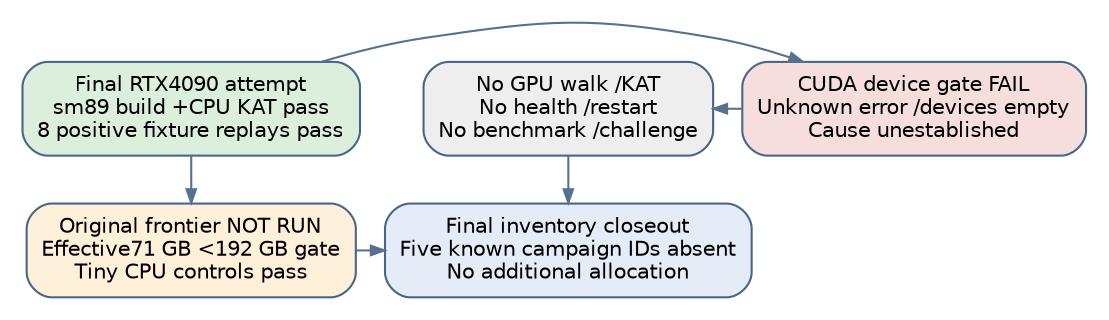
\includegraphics[width=\linewidth]{gpu-final-flow.png}

\textbf{Observed passes and failed device gate.} CUDA13.3.73 compiles the
client for compute89/sm89. CPU controls pass 48/48 known answers, 2,862 sigma,
28,645 CLMUL and 28,642 portable checks. The remote corrected-ingester positive
fixture passes 8 records/8 golden replays; no zero-length case is in that fixture.
Device initialization exits 3 with CUDA unknown error, driver API 13000,
runtime 13030 and an empty device list. Native GPU KAT/checker, GPU walk,
GPU-report ingestion, health/restart, throughput samples and challenge
collection do not run.

\texttt{nvidia-smi} reports driver 580.126.09 and GPU Recovery Action Reboot.
The cause of initialization failure remains \textbf{unknown}. That field alone
is not a physical-hardware diagnosis; general toolchain incompatibility is
not established. Build/CPU fixture passes are not GPU arithmetic validation.

\textbf{Frontier and negation.} Physical RAM 540,788,072,448bytes, effective
cgroup 70,999,998,464bytes; the 192,000,000,000-byte gate exits 78. Tiny SAT/UNSAT
controls pass, but the original large n19/m3/ell7,draw0,degree5 closure does
not execute. No new D or memory-frontier measurement is supplied. Baseline
negation reports a collision flag at 42,678 steps; the three quotient arms
are censored at 2,208,379 steps. No recovered-scalar certificate or gain follows.

\textbf{Evidence and cleanup.} Archive 27,318 bytes, SHA256 prefix
\texttt{d74c3fab830939e3}. All 120 manifest-listed payload files verify in
retained and fresh trees with exact coverage; 121 archived files include the
manifest. Raw records remain unchanged. Controller outcome records fetch,
exact-ID deletion and absence. Root's separate complete one-page API-v2
inventory finds all five known allocated campaign IDs absent and zero
campaign-prefix resources; a separate exact latest-ID GET returns 404.
The detached local watchdog is state Z (stopped, not running), not claimed
absent. No further allocation follows. Receipt:
\path{resource-runs/gpu-final-01/root-final-inventory.json}.

\textbf{Unchanged scope.} The prior five-page PDF is preserved as
\path{reports/CPU-api-v2-report.pdf}, hash prefix \texttt{70b17e44201e6dff}.
Full record: \texttt{GPU\_FINAL\_RESULTS.md}. Run1's short control and local
ingestion qualification remain scoped; production rates/forecasts, IC
leaderboard and scientific status stay unchanged. This closes the bounded
resource attempt, not the missing healthy-device, restart, benchmark,
challenge-scalar or original large-closure obligations.
